\documentclass[conference]{IEEEtran}

%% Document properties (~ is a non-breaking space)
\title{Using Factored~Weight~Matrices for an efficient SpiNNaker implementation of the Neural~Engineering~Framework}
\author{%
  \IEEEauthorblockN{Andrew~Mundy, James~Knight and Steve Furber}
  \IEEEauthorblockA{School of Computer Science,\\
                    University of Manchester,\\
                    Oxford Road, Manchester,\\
                    M13 9PL, UK\\
                    Email: andrew.mundy@ieee.org}
  \and
  \IEEEauthorblockN{Terry Stewart}
  \IEEEauthorblockA{Centre for Theoretical Neuroscience,\\
                    University of Waterloo,\\
                    Waterloo, ON,\\
                    Canada N2L 3G1\\
                    Email: tcstewar@uwaterloo.ca}
}

%% Utilities
\usepackage{booktabs}  %% Pleasant tables
\usepackage[binary-units]{siunitx}
\usepackage[caption=false, font=footnotesize]{subfig}
\usepackage{graphicx}

%% Source highlighting
\usepackage{listings}
\lstset{
  language=Python,
  morekeywords={with,as},
  columns=flexible,
  gobble=2,
  basicstyle=\footnotesize,
  xleftmargin=1em,
}

%% Maths
\renewcommand{\vec}{\mathbf}  % Bold vectors

%% Bibliographies
\usepackage[backend=bibtex, style=ieee, doi=false, url=false]{biblatex}
\bibliography{paper}
\usepackage{xcolor}

\begin{document}
  \maketitle

  \begin{abstract}

Building and simulating neural systems is a promising avenue in our search for understanding how the brain may work and for how neural and cognitive systems may be employed to tackle engineering problems. The Neural Engineering Framework (NEF) is an interesting hypothesis about how such systems may be constructed and has recently being used to build the world's first functional brain model. However, while the NEF simplifies the design of complex neural networks, simulating these using standard computer hardware is still computationally expensive -- often running far slower than biological real-time and scaling very poorly: problems the SpiNNaker neuromorphic simulator was designed to solve. In this paper we (1) argue that employing the model of computation used for simulating general purpose spiking neural networks on SpiNNaker for NEF models is sub-optimal, and (2) provide and evaluate an alternative simulation scheme which overcomes the memory and communication challenges posed by the NEF.

  \end{abstract}

  \section{Introduction}

For a given power budget, two factors limit the simulation of neural networks on any computing platform: scale and time. In principle any scale of network may be simulated but as scale increases simulation time follows. Conversely, if the simulation time is limited (for example, if biological real-time is necessary) then only a limited scale of network may be simulated. Specialised ``neuromorphic'' hardware tries to avoid these constraints by parallelising and distributing computational effort and relying on dense interconnection of the computing elements. The SpiNNaker platform \parencite{Furber2014} is one of a range of neuromorphic simulators (including NeuroGrid \parencite{}, FACETS \parencite{} and lately TrueNorth \parencite{}) which should benefit investigators of embodied cognition and researchers of large neural models alike by enabling scalable, rapid simulation of large-scale neural networks.

The Neural Engineering Framework (NEF) \parencite{Eliasmith2004} is a hypothesis about how neurons may act to encode the abstract mathematical constructs, such as scalars and vectors, that we often use in modelling the real world. Its successes so far include the Spaun model of cognition \parencite{Eliasmith2012} and applications in embedded robotics (e.g., \parencite{Stewart2015ip}). As with all neural systems, the NEF has proven costly to simulate with simulations of the Spaun model typically taking \SI{2.5}{\hour} of simulation time for \SI{1}{\second} of simulation \parencite[\S V]{Stewart2014}. Two aspects of NEF networks that make them particularily costly to simulate are the high firing rates of individual neurons (around \SIrange{200}{400}{\hertz} when saturated) and the dense synaptic matrices used to connect neuronal populations. The former presents a significant communication cost to any specialised neuromorphic hardware and the latter requires that large amounts of memory be used to represent the neural network with all the associated costs of transferring large blocks of data that implies.

  In this paper we:
  \begin{enumerate}
    \item argue that due to these properties of the NEF, the existing solutions and algorithms used to simulate neural networks on SpiNNaker will not satisfactorily scale to Spaun-like models,
    \item detail a method by which features of the NEF may be used to reduce the communication and memory costs associated with its simulation.
  \end{enumerate}

The result is a model of computation similar to the data-flow computer which we hope to use in running the full Spaun model in biological real-time.

  \section{Background}

In this section we briefly discuss the SpiNNaker platform and how neural networks are currently simulated on it before introducing the Neural Engineering Framework (NEF) and discussing how models built with it may act to stress SpiNNaker in various ways.

  \subsection{The SpiNNaker platform}

The SpiNNaker platform is a massively parallel architecture designed to simulate neural networks. A SpiNNaker machine is constructed from a number of SpiNNaker chips, each connected to their six immediate neighbours using a chip-level interconnection network with a toroidal, triangular mesh topology. Each SpiNNaker chip contains 18 ARM processing cores connected, via a network-on-chip, to each other and the external network through a multicast router. Each core has two small tightly-coupled memories: \SI{32}{\kibi\byte} for instructions~(ITCM) and \SI{64}{\kibi\byte} for data~(DTCM) and shares \SI{128}{\mebi\byte} of off-chip SDRAM with the other cores on the SpiNNaker chip.

SpiNNaker is an event-driven message-passing computing architecture. The software running on a core may transmit packets to other processing cores to indicate the occurrence of events or to share data. A packet consists of a \SI{32}{\bit} key -- which is used to direct the packet around the network -- and, optionally, a \SI{32}{\bit} data payload. When a packet reaches a router the key is inspected to determine to which (if any) of the 18 processors and six external links attached to the router it should be forwarded. On receipt of a packet a core executes a \textit{callback} function which may inspect the packet and schedule further execution as required.

  \subsection{Simulating neural nets on SpiNNaker}
  \label{sef:background/nn}

When simulating neural nets on a SpiNNaker machine, each core is responsible for simulating a number (in the order of a few hundred) of point neurons. When one of these neuron spikes, it transmits a packet whose key uniquely identifies the neuron (for this it requires no payload). This ``spike'' packet is then routed across the network fabric to the processing cores responsible for simulating each of the neurons that are synaptically connected to the firing neuron. On receipt of a ``spike'' packet, a core retrieves the row of the connectivity matrix associated with the firing neuron from SDRAM. Each of these rows describes the synaptic weights and delays associated with the connections between the firing neuron and those simulated on the core. Once a row is retrived, the weights are inserted into an input ring-buffer where they remain until the synaptic delay has elapsed and they are used to calculate the neuronal input current.

There are three primary constraints to the number of neurons that may be simulated on a single processing core:

  \begin{enumerate}
    \item The amount of memory required to store the synaptic weight matrices must fit within the space available to the core.
    \item The number of packets likely to be transmitted by the core should not lead to saturation of the interconnection network.
    \item As \textcite{Sharp2013} discuss, the majority of processing time is spent in the synaptic processing pipeline so there must be sufficient time for the core to process all incoming `spike' packets; and retrieve and process the synaptic rows during one simulation time-step.
  \end{enumerate}

These constraints may be met by either allocating fewer neurons to each processing core or by increasing the processing time used for each simulation time-step.

In practice there are limits to the number of processors and the amount of time that are available (though one aim of the SpiNNaker project is to build a machine consisting of one million cores). Hard time constraints are necessary when SpiNNaker is required to run in biological real-time, as it is in experiments with other neuromorphic hardware. Processor constraints are present for those with access to only small SpiNNaker machines. At some point it is necessary to ensure that efficient use is made of the machine with regard to both time and processor usage.

To a first approximation the first constraint is that the synaptic matrices for a core's neurons must fit within $\frac{128}{16} = \SI{8}{\mebi\byte}$. The interconnection network was designed around an expectation that each core would simulate around \num{1000} neurons firing at roughly \SI{10}{\hertz} and that consequently the second constraint is that when simulating on a millisecond time-step in biological real-time each core is expected to transmit around 10 spikes per time-step. The third constraint is given by \textcite[\S III.C]{Sharp2013} as around \num{5000} spikes per millisecond.

It should be noted that time is also a factor \textit{prior} to the start of any simulation. All data required by the SpiNNaker machine during simulation must be transmitted to it across ethernet, consequently the more data required on the machine the greater the time required to prepare it for simulation. \textcite{Sharp2013} note that this can take a significant period of time and that this is undesirable if a real-time simulator is desired.

  \subsection{The Neural Engineering Framework}

The Neural Engineering Framework (NEF) extends the concept of ``preferred-direction vectors'' \parencite{} to all neural populations. Each population is said to represent a vector within a particular space, with each neuron in that population firing in response to the similarity of the represented vector to its own ``encoding'' vector.  Using the notation of \textcite{Stewart2014} this may be expressed as:

\begin{equation}
  \delta_{i}\left(\vec{x}\right) = G_{i}\left[ \alpha_i \vec{e}_i \cdot \vec{x} + J^{bias}_i \right]
\end{equation}

Which states that the firing response of neuron $i$, $\delta_i$, to the represented value of $\vec{x}$ is the response of the neuron model to an input consisting of a randomly selected gain term ($\alpha_i$), the encoding vector for the neuron ($\vec{e}_i$) and a fixed bias current $J^{bias}_i$.  The process of ``encoding'' allows us to transform a variable in vector form into the spiking response of a population of neurons.  Correspondingly, ``decoding'' allows a transformation from the spiking actions of neurons into the domain of vectors.  Again using the notation of \textcite{Stewart2014} we can express this decoding process as:

\begin{equation}
  \vec{\hat{x}} = \sum\limits_{i=1}^{N} a_i(\vec{x})\vec{d}_i  \label{eq:decoding}
\end{equation}

Where the estimate of the original represented value $\vec{\hat{x}}$ is the sum of the spiking activity of each neuron $a_i$ multiplied by the linear decoder for the neuron $\vec{d}_i$.  The decoding vectors $\vec{d}_i$ may be selected to compute a function of the value represented by the population.  \figurename \ref{fig:background/nef-1} illustrates the encoding of a two-dimensional value using four neurons -- the role of the encoding vectors can be seen in that each neuron becomes active for only a small range of the input space.

  \begin{figure}[!t]
    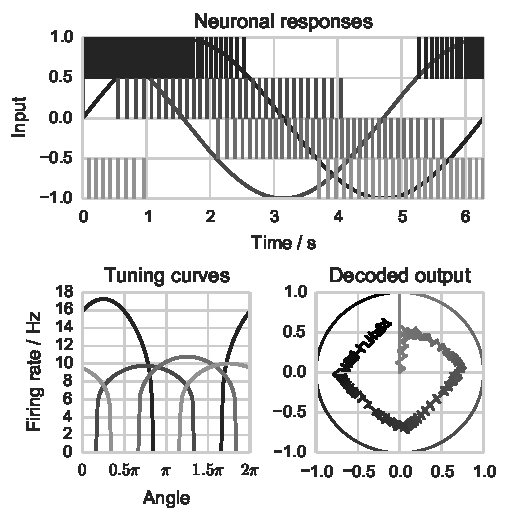
\includegraphics{nef-1}
    \caption{Representing a 2-dimensional value using four neurons.  The input values and spiking responses of the neurons are shown in the top plot.  The bottom left-hand plot shows how the firing responses vary to the angle of the 2-D input vector (tuning curves) and the bottom right-hand plot shows a decoding of the population's representation along with the input value.}
    \label{fig:background/nef-1}
  \end{figure}

%% Synaptic filtering

The combination of encoders and decoders leads naturally to the connection weights between any pair of neuronal populations. For a connection between a pair of populations the synaptic weights are given by the matrix product of the decoders of the pre-synaptic population and the encoders of the post-synaptic population \parencite{Stewart2014}:

\begin{equation}
  \omega_{ij} = \alpha_j \vec{d_i}\vec{e_j}
\end{equation}

With $i$ indexing neurons in the pre-synaptic population and $j$ those in the post-synaptic population.  The resultant connection matrix will typically be dense.

  \subsection{Assessing the Neural Engineering Framework (NEF)}

  TODO: Compare known facts about the NEF to SpiNNaker constraints.

  \subsection{Constructing models with the NEF}

Neural models built using the principals of the NEF may be implemented in any programming language, however, a standard Python library for building and simulating these models has been developed.  Nengo \parencite{Bekolay2014} provides several core components which may be used to specify models for simulation:

  \begin{description}[\IEEEsetlabelwidth{Connections}]
    \item[Ensembles] A population of neurons with their attendant encoders.
    \item[Nodes] General purpose non-neural components, typically used to inject values into simulations or to drive real-world actuators.
    \item[Connections] Specify how nodes and ensembles are connected.
    \item[Probes] Allow gathering of simulation data for later analysis.
  \end{description}

  An illustrative model that we will use later in this paper is the \textit{communication channel}.  A communication channel consists of two ensembles connected with the synaptic weights chosen such that the second ensemble will represent the same value as the first ensemble.  The concept is illustrated in \figurename~\ref{fig:background/comms-channel}.  Using Nengo a communication channel may be constructed as:

  \begin{lstlisting}
  with nengo.Network('Communication Channel') as comms_channel:
      # 2 100 neuron ensembles, each of 2-dimensions
      ens_a = nengo.Ensemble(100, 2)
      ens_b = nengo.Ensemble(100, 2)

      # Connection from A to B with the identity function
      nengo.Connection(ens_a, ens_b)
  \end{lstlisting}

  \section{Exploiting features of the NEF for effective simulation on SpiNNaker}

Previous sections discussed the manner in which neural networks are typically simulated on the SpiNNaker hardware, introduced the Neural Engineering Framework and have indicated the ways in which the NEF exceeds the design specification of the SpiNNaker hardware and software model.  In this section we review an alternative simulation scheme that will meet the constraints of the SpiNNaker hardware for a large range of networks constructed using the NEF.

The NEF permits us two different views of the activity of a neural population: that of spikes and that of a set of time-varying vectors.  In our simulation scheme we use the second of these to facilitate communication of neural activity between processing cores.  Considering the simple example of \figurename~\ref{fig:background/nef-1}, at each time-step the current activity of the population can be represented as either two values for the immediate decoding of the population or between zero and four values representing the indices of spiked neurons. Using the former (value-based) representation rather than the latter (spike-based) is beneficial as (1) in the majority of cases it will result in the transmission of fewer packets across the SpiNNaker network, and (2) less memory is required to store the vectors used for decoding and encoding values than would be required to store the weight matrices of every connection.  Reducing network usage reduces the likelihood of causing network links to become blocked, reducing the memory requirements of a simulation allows an increase in the number of neurons which may be simulated on a core and a reduction in the time required to load data on the SpiNNaker machine.  These gains are indicated by results in \S\ref{sec:results}.

  \subsection{Simulating neurons}

As when simulating standard neural nets on SpiNNaker (\S\ref{sef:background/nn}) each processing core is assigned a number of point neurons.  When one of these neurons fires the decoder vector for the neuron is looked up and added to a buffer storing the immediate decoding of the population (see (\ref{eq:decoding})).  Once per time-step each element of the buffer is transmitted in the payload of a multicast packet to all the cores which receive connections from this population.  The key of one of these ``value'' packets is constructed such that the packet reaches all intended cores and that the index of the element of the vector can be deduced.  On receipt of a value-packet a core inspects the key to determine in which synaptic filter the value should be included and to which element it should be added.  At the start of the next simulation time-step the synaptic filters are executed to generate the current input to the ensemble.  On simulating each neuron the current input is encoded using that neuron's encoding vector to form the input to the neuron.

  \subsection{Injecting and retrieving values}

  \section{Results}
  \label{sec:results}

  \subsection{Processor utilisation}

  \textbf{Processor utilisation for communication channel (show variation with dimensionality and neuron count) \color{red} Jamie}

  \subsection{Network utilisation}

  \textbf{Network utilisation for communication channel, varying neuron count and dimensionality \color{red} Andrew}

  \begin{figure}[!t]
    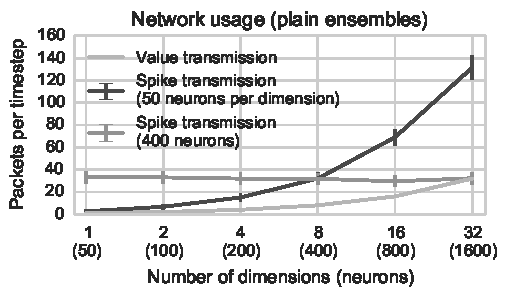
\includegraphics{network-1}
    \caption{}
    \label{fig:results/network-utilisation}
  \end{figure}

  \subsection{Memory utilisation}

  \textbf{Memory utilisation for comms channel and basal ganglia model with varying scale \color{red} Andrew}

  \subsection{Simulating large-scale models}

  \textbf{Simulation results from SPA sequence, indicate compute/load time \color{red} Both, discuss first.}

  \section{Discussion}

  \section{Conclusion}

  \section*{Acknowledgements}

The authors would like to extend their thanks to the organisers of the Telluride Neuromorphic Cognition Engineering Workshop.

The research leading to these results has received funding from the European Research Council under the European Union’s Seventh Framework Programme (FP7/2007-2013) / ERC grant agreement number 320689.

  \printbibliography

\end{document}
